\documentclass[11pt,a4paper]{article}

\usepackage[T1]{fontenc}
\usepackage[utf8]{inputenc}
\usepackage{lmodern}
\usepackage{microtype}
\usepackage{amsmath,amssymb}
\usepackage{graphicx}
\usepackage{xcolor}
\usepackage{hyperref}
\usepackage{xurl}  % break long URLs anywhere, so the availability paragraph
                   % does not leave underfull (loose) lines around GitHub links
\usepackage{natbib}
\usepackage{geometry}
\usepackage{caption}
\usepackage{algorithm}
\usepackage{algpseudocode}
\usepackage{parskip}
\usepackage{upquote}  % straight quotes in verbatim, so the code can be pasted
\usepackage{tikz}
\usetikzlibrary{arrows.meta, positioning, calc}

\geometry{margin=2.5cm}

% Absorb hard-to-break lines (long \texttt package names, DOI URLs) into
% slightly looser spacing instead of letting them bleed into the margin.
\setlength{\emergencystretch}{3em}

% Benchmark macros, generated by src/coxbench/gen_arxiv_macros.py from
% results/competing_coxph.json et al. Do not hand-edit paper_macros.tex.
% GENERATED by src/coxbench/gen_arxiv_macros.py -- do not
% edit by hand. Regenerate after a benchmark re-run:
%   python3 -m coxbench.gen_arxiv_macros
% Speed/RAM macros track the host that wrote competing_coxph.json; the
% recovery-error, coef-gap and tie macros are platform-independent.

\newcommand{\CoxPHNSweepP}{10}
\newcommand{\CoxPHPSweepN}{1\,000\,000}
\newcommand{\CompetingCoxPHN}{4\,000\,000}
\newcommand{\CoxStreamRAMLoN}{1\,000\,000}
\newcommand{\CoxStreamRAMHiN}{32\,000\,000}
\newcommand{\CoxStreamRAMNFactor}{32}
\newcommand{\CoxPHRAMRatioN}{16\,000\,000}
\newcommand{\CoxPHPLo}{8}
\newcommand{\CoxPHPHi}{128}
\newcommand{\CoxStreamMaxErr}{3.39 \times 10^{-3}}
\newcommand{\CoxStreamMaxErrSE}{1.9}
\newcommand{\CyclopsMaxErr}{3.39 \times 10^{-3}}
\newcommand{\CoxStreamErrLoP}{1.16 \times 10^{-1}}
\newcommand{\CoxStreamErrHiP}{8.20 \times 10^{-3}}
\newcommand{\CoxStreamVsLifelinesCoef}{2.56 \times 10^{-14}}
\newcommand{\CoxStreamVsLifelinesSERel}{4.37 \times 10^{-13}}
\newcommand{\CyclopsVsLifelinesCoef}{6.61 \times 10^{-10}}
\newcommand{\TiesN}{3\,000\,000}
\newcommand{\TiesSubN}{20\,000}
\newcommand{\TiesRowGroupMin}{1\,000}
\newcommand{\TiesNTieGroups}{120}
\newcommand{\TiesMaxGroupEvents}{8\,170}
\newcommand{\TiesStreamVsEfronCoef}{1.55 \times 10^{-11}}
\newcommand{\TiesStreamVsEfronSERel}{7.07 \times 10^{-12}}
\newcommand{\TiesStreamVsNumpyCoef}{5.11 \times 10^{-15}}
\newcommand{\TiesRVsLifelinesCoef}{1.55 \times 10^{-11}}
\newcommand{\TiesStreamVsLifelinesCoef}{5.48 \times 10^{-13}}
\newcommand{\TiesBresVsEfronMonthly}{1.35 \times 10^{-3}}
\newcommand{\TiesBresVsEfronYearly}{1.53 \times 10^{-2}}
\newcommand{\CoxStreamIters}{5}
\newcommand{\CoxStreamPasses}{6}
\newcommand{\CoxStreamReps}{5}
\newcommand{\BaselineReps}{2}
\newcommand{\WallSpreadPct}{5.1}
\newcommand{\RAMSpreadPct}{7.1}
\newcommand{\CoxStreamChunkRows}{200\,000}
\newcommand{\RSSPollMs}{50}
\newcommand{\DGPShape}{1.5}
\newcommand{\DGPCensRate}{0.04}
\newcommand{\DGPFollowUp}{10}
\newcommand{\DGPCoefMin}{0.01}
\newcommand{\DGPCoefMax}{0.5}
\newcommand{\DGPExtraCoef}{0.1}
\newcommand{\LifelinesVsCoxStreamSpeedup}{34.8}
\newcommand{\CoxStreamVsCyclopsSpeedup}{1.9}
\newcommand{\CyclopsVsLifelinesSpeedup}{18.3}
\newcommand{\CyclopsRAMRatio}{7.8}
\newcommand{\RSurvivalRAMRatio}{8.0}
\newcommand{\CoxStreamRAMMinGB}{0.39}
\newcommand{\CoxStreamRAMMaxGB}{0.45}
\newcommand{\LifelinesRAMGB}{9.2}
\newcommand{\ExtrapN}{10^{8}}
\newcommand{\LifelinesRAMExtrapGB}{55}
\newcommand{\CoxStreamTol}{10^{-8}}
\newcommand{\CoxStreamMaxIter}{50}
\newcommand{\CoxStreamMaxHalvings}{15}
\newcommand{\CoxStreamLLRtol}{10^{-12}}
\newcommand{\CoxStreamRMaxIter}{25}
\newcommand{\EnvMachine}{n2-standard-8}
\newcommand{\EnvVCPUs}{8}
\newcommand{\EnvCores}{4}
\newcommand{\EnvCPU}{Intel Xeon (Cascade Lake) at 2.8\,GHz}
\newcommand{\EnvRAMGB}{32}
\newcommand{\EnvDiskGB}{100}
\newcommand{\EnvUbuntu}{24.04}
\newcommand{\EnvPython}{3.13.16}
\newcommand{\EnvNumPy}{2.5.3}
\newcommand{\EnvSciPy}{1.18.1}
\newcommand{\EnvPyarrow}{25.0.1}
\newcommand{\EnvLifelines}{0.30.3}
\newcommand{\EnvR}{4.3.3}
\newcommand{\EnvSurvival}{3.5.8}
\newcommand{\EnvCyclops}{3.7.1}
\newcommand{\EnvRBLAS}{the reference BLAS}


\hypersetup{
    colorlinks=true,
    linkcolor=blue!60!black,
    citecolor=blue!60!black,
    urlcolor=blue!60!black,
    pdftitle={CoxStream: Out-of-Core Cox Proportional Hazards
              Regression by Streaming Newton\textendash Raphson},
    pdfauthor={Tommy Carstensen and Clara S. Gr\o nkj\ae r},
    pdfsubject={Survival analysis; out-of-core estimation},
    pdfkeywords={Cox proportional hazards; survival analysis; out-of-core;
                 streaming; Newton\textendash Raphson; Efron;
                 partial likelihood},
}

\newcommand{\x}{\ensuremath{\times}}
\newcommand{\coxstream}{\textsc{CoxStream}}

% ============================================================
\title{\coxstream: Out-of-Core Cox Proportional Hazards
       Regression by Streaming Newton--Raphson}

\author{Tommy Carstensen\\
        \small \texttt{arxiv@tommycarstensen.com}\\[2pt]
        \small \href{https://orcid.org/0000-0002-3672-9931}
                    {ORCID: 0000-0002-3672-9931}
        \and
        Clara S. Gr{\o}nkj{\ae}r\\[2pt]
        \small \href{https://orcid.org/0000-0001-7739-1917}
                    {ORCID: 0000-0001-7739-1917}}

\date{\today}
\widowpenalty=10000
\clubpenalty=10000
% ============================================================

\begin{document}
\maketitle

\begin{abstract}
Standard Cox proportional hazards solvers load the full design matrix
and event times into memory before fitting, so the memory they need grows
linearly with the cohort and can exceed a workstation's RAM on registry-scale
data. We
present \coxstream, an estimator that maximises the same Efron partial
likelihood as in-memory solvers by streaming a time-sorted Parquet file (an
on-disk table format) chunk by chunk, once per Newton--Raphson iteration, while
holding only $O(p^2)$ running sums for $p$ covariates plus the chunk in hand.
Working memory is therefore
independent of the number of observations $n$: across $n = \CoxStreamRAMLoN$ to
$\CoxStreamRAMHiN$ rows it is essentially constant, while \texttt{lifelines}
grows with $n$ and by $n = \CoxPHRAMRatioN$ uses more than an order of magnitude
more. \coxstream\ reproduces the in-memory estimate to near machine precision
(maximum coefficient gap $\CoxStreamVsLifelinesCoef$\ versus \texttt{lifelines}),
carries the Efron tie correction exactly across chunk boundaries, and returns
model-based standard errors from the same pass. Its input must first be sorted
by descending time, a one-off step outside our measurements. At $p =
\CoxPHNSweepP$ it was also the fastest method at every $n$ we ran,
\CoxStreamVsCyclopsSpeedup\ times faster than \texttt{Cyclops} at $n =
\CompetingCoxPHN$. The method covers the right-censored Cox model with fixed
covariates; strata, delayed entry, time-varying covariates and case weights
are not yet supported.
\end{abstract}

% ============================================================
\section{Introduction}
\label{sec:intro}

The Cox proportional hazards model \citep{cox1972regression} is the workhorse of
time-to-event analysis. Its partial likelihood ties every observation to the
rest through the \emph{risk set} at each event time $t_i$, the subjects
$\{j : t_j \ge t_i\}$ still under observation when $i$'s event occurs. The
standard fitting recipe reads all rows into a data frame and then iterates
Newton--Raphson over the in-memory design matrix, which needs $O(np)$ memory.
For linked administrative health registries, national cancer registries, and
electronic-health-record cohorts, where $n$ routinely reaches $10^7$--$10^8$
rows with modest $p$, that requirement is the binding constraint: the model is cheap,
but the data do not fit. The remedy is to fit \emph{out of core}: leave the rows
on disk and read them in chunks small enough to hold in RAM, so that working
memory no longer scales with the cohort. Throughout, an \emph{exact} fit is one
that maximises the same partial likelihood, with the same Efron handling of
tied event times, as an in-memory solver, rather than a stochastic, subsampled
or surrogate objective; Efron's formula itself approximates the partial
likelihood when event times are tied \citep{efron1977efficiency}, and we claim
nothing beyond agreement with it.

\coxstream\ \citep{coxstream2026} is an exact out-of-core fit in that sense. It
runs the classical descending-time pass over the risk sets on a chunked file,
with an $O(p^2)$ carry state and a tie group carried across chunk boundaries,
so that each Newton--Raphson iteration needs only $O(p^2)$ running sums and the
data are never held in full. The pass itself is not new; the contribution is
its out-of-core form, a released implementation in Python and R, and the
measurements. The estimate agrees with the in-memory fit to near machine
precision; only the memory profile differs, staying flat in $n$,
whereas the footprint of in-memory solvers grows linearly with $n$
(Figure~\ref{fig:ram}). The method covers the right-censored Cox model with
fixed covariates; left truncation (delayed entry), time-varying covariates,
strata and case weights are outside its current scope
(Section~\ref{sec:discussion}).

To our knowledge, no other released tool computes the exact unpenalised Efron
fit from a file on a single machine in working memory independent of $n$. The
in-memory exact solvers
(\texttt{lifelines} \citep{davidsonpilon2019lifelines} and R's
\texttt{survival} \citep{therneau2000modeling}) both load
the whole cohort into RAM before fitting. Tools built for massive sample sizes
stay in memory too: \texttt{Cyclops} fits Cox by cyclic coordinate descent over
sparse, column-major data structures \citep{mittal2014highdim} that shrink the
footprint for high-dimensional sparse covariates, most often with
regularisation. It also offers an unpenalised maximum-likelihood mode, but it
still holds the encoded cohort in RAM and is not aimed at dense out-of-core
streaming. Approximate scalable methods relax the objective:
\texttt{BigSurvSGD} \citep{tarkhan2020bigsurvsgd,tarkhan2024online} restricts
each risk set to a small random stratum and optimises by stochastic gradient
descent (SGD), so each update touches few rows; its result is a stochastic
approximation, not the maximiser of the full partial likelihood, and we do not
benchmark it here. Cluster
solvers (e.g.\ \texttt{h2o.coxph}) require a Java virtual machine and an
in-memory distributed frame, not a streaming-from-disk workflow. In-database
libraries are another route: Apache MADlib \citep{hellerstein2012madlib} fits
the Cox model by Newton--Raphson inside a PostgreSQL or Greenplum database,
with the Breslow tie correction; the cohort must first be loaded into such a
database, and we did not evaluate it. A separate
line of work fits streaming generalised linear models (GLMs) by renewable
estimation, updating sufficient statistics as data arrive without revisiting
them \citep{luo2020renewable}. The GLM log-likelihood is a sum
of independent per-observation terms, whereas the Cox partial likelihood
couples every observation through the shared risk set, so those incremental
updates do not carry over in exact form. A sizeable literature attacks the
resulting bottleneck, but only by relaxing the coupling: discretising the
baseline hazard into piecewise-constant intervals \citep{wu2021online},
restricting risk sets to small strata for stochastic-gradient training
\citep{tarkhan2024online}, replacing the partial likelihood with a full
likelihood whose baseline hazard is a Bernstein polynomial, which avoids risk
sets altogether \citep{hu2024privacy}, requiring the whole cohort up front for
divide-and-conquer \citep{wang2021divide} or subsampling \citep{qiao2023optimal},
or updating a subsample fit by one Newton step over the remaining data, which
is asymptotically, not numerically, equivalent to the maximum-likelihood
estimate (MLE) \citep{wang2024fitting}. None of these reduces the
continuous-time partial likelihood to a fixed-size, revisit-free summary the
way the GLM case admits; the risk-set coupling is what each of them works
around.

Other tools lower the memory footprint in other ways. The descending-time
cumulative-sum evaluation of the risk-set power sums that our pass rests on is
the classical in-memory Cox computation \citep{therneau2000modeling};
\texttt{Cyclops}'s recent graphics-processor (GPU) implementation runs it as a
parallel scan \citep{yang2023massive} and extends to stratified and
time-varying Cox models \citep{yang2023gpu}; both papers address speed through
parallelism, and out-of-core data access is not their subject.
Penalised high-dimensional
solvers reach out of
core by memory-mapping: \texttt{biglasso} \citep{zeng2021biglasso} and
\texttt{snpnet-Cox} \citep{li2022snpnet} fit $L_1$-regularised Cox models on data
larger than RAM, but they target ultra-high-dimensional screening by batched
coordinate descent rather than the exact unpenalised MLE in one pass per
Newton step, and their working memory is not bounded
independently of $n$. We did not evaluate commercial procedures such as SAS
\texttt{PROC PHREG} or Stata's \texttt{stcox}; their source is closed, so their
memory behaviour cannot be inspected. Recent work also speeds up the in-memory
fit itself \citep{liu2024fastsurvival} without addressing where the data live.
Finally, the exact reduction of the risk-set-coupled partial likelihood to
recombinable summary statistics is known from federated learning:
\texttt{WebDISCO} \citep{lu2015webdisco} exchanges local risk-set aggregates
across institutions to fit a Cox model provably identical to the pooled one,
but it is designed for exchange between institutions, not for streaming one
file from disk on a single machine. One-shot distributed methods instead
approximate the pooled partial likelihood with a surrogate built from site
summaries \citep{duan2020odac}, and SAS-based distributed implementations fit
Cox models from site-level summary statistics \citep{vilk2018sas}.

% ============================================================
\section{Method}
\label{sec:method}

Let $(t_i, \delta_i, \mathbf{x}_i)_{i=1}^n$ be event/censoring times, event
indicators $\delta_i \in \{0,1\}$ ($\delta_i = 1$ if subject $i$ is observed to
have the event at $t_i$, and $0$ if the subject is censored there), and
covariates $\mathbf{x}_i \in \mathbb{R}^p$. The Cox model writes the hazard of
subject $i$ at time $t$ as
\begin{equation}
    h(t \mid \mathbf{x}_i)
        = h_0(t)\,\exp(\mathbf{x}_i^\top\boldsymbol\beta),
    \label{eq:hazard}
\end{equation}
an unspecified \emph{baseline hazard} $h_0$ shared by everyone, multiplied by a
subject-specific factor that does not vary with time. The baseline cancels from
the ratio of hazards within a risk set, which is why $\boldsymbol\beta$ can be
estimated from the partial likelihood without ever estimating $h_0$. For
distinct event times, the partial log-likelihood scores each event against the
covariates of everyone still at risk when it occurs:
\begin{equation}
    \ell(\boldsymbol\beta) = \sum_{i:\,\delta_i=1}
        \Bigl[\mathbf{x}_i^\top\boldsymbol\beta
              - \log S_0(t_i;\boldsymbol\beta)\Bigr],
    \qquad
    S_0(t;\boldsymbol\beta) = \sum_{j:\,t_j \ge t}
        \exp(\mathbf{x}_j^\top\boldsymbol\beta),
    \label{eq:cox}
\end{equation}
where $S_0$ sums the hazard weights $\exp(\mathbf{x}_j^\top\boldsymbol\beta)$
of the risk set (ties at a shared event time are handled below). The score
$\mathbf{g} = \partial\ell/\partial\boldsymbol\beta$ and the observed information
$H = -\partial^2\ell/\partial\boldsymbol\beta\,\partial\boldsymbol\beta^\top$,
the negative Hessian of $\ell$ that Newton--Raphson needs and that also gives
the standard errors, depend on the data only through three running sums over the
risk set $R(t) = \{j : t_j \ge t\}$:
\begin{equation}
    S_0(t) = \sum_{j \in R(t)} w_j, \qquad
    S_1(t) = \sum_{j \in R(t)} w_j\,\mathbf{x}_j, \qquad
    S_2(t) = \sum_{j \in R(t)} w_j\,\mathbf{x}_j\mathbf{x}_j^\top,
    \label{eq:powersums}
\end{equation}
with weights $w_j = \exp(\mathbf{x}_j^\top\boldsymbol\beta)$, so that
$S_0(t) \in \mathbb{R}$, $S_1(t) \in \mathbb{R}^p$, and
$S_2(t) \in \mathbb{R}^{p \times p}$; $\mathbf{g}$ and $H$ are closed-form
functions of them, written out in Appendix~\ref{app:derivation}. Together with
the moments of the currently open tie group (below) and the running $\ell$,
$\mathbf{g}$ and $H$, these sums are the whole state the streaming pass
carries: a fixed number of vectors and $p \times p$ matrices. The same sums give the baseline:
the Breslow estimator
$\hat{\Lambda}_0(t) = \sum_{i:\,\delta_i=1,\,t_i \le t} 1/S_0(t_i;\hat{\boldsymbol\beta})$
of the cumulative baseline hazard \citep{breslow1974covariance} needs only $S_0$
at the estimate, which one further pass provides; the current packages do not
expose it.

\paragraph{Streaming accumulation.} Once the data are in descending time
order, the risk set $R(t_i)$ consists of exactly the rows read up to and
including the last row at time $t_i$, so the $S_r$ can be accumulated as
running sums: read from the latest time backward, each new row joins the
at-risk group and never leaves it, so the sums only grow and nothing is
recomputed. A censored row tied with an event belongs to that event's risk set
($t_j \ge t_i$), and the order of the rows within one time does not matter,
because a time's contribution is added only once a strictly earlier time
arrives. One descending pass over the data therefore yields $\ell$,
$\mathbf{g}$ and $H$ at the current $\boldsymbol\beta$, accumulating a carry
state of size $O(p^2)$ plus a single \emph{chunk} in flight: a block of
consecutive rows, the unit in which the file is read (in the Python package,
one Parquet row group). The Cox partial log-likelihood is concave, so $H$ is
positive semidefinite, and positive definite when the covariates are not
collinear over the risk sets of the observed events; the Newton direction
$\Delta = H^{-1}\mathbf{g}$, obtained from the small $p \times p$ solve
$H\Delta = \mathbf{g}$, is then an ascent direction. A finite maximiser can
fail to exist when the data are separated (a covariate combination perfectly
orders the events), and the iteration then diverges.

In the Python package, the update $\boldsymbol\beta \leftarrow
\boldsymbol\beta + \alpha\,\Delta$ takes the full step $\alpha = 1$ unless that
lowers $\ell$ by more than a relative slack of $\CoxStreamLLRtol$ of $|\ell|$,
set at the rounding level of the summed log-likelihood; otherwise $\alpha$ is
halved, at most \CoxStreamMaxHalvings\ times (step-halving), and if every trial
fails the smallest step is taken. Each trial point costs one streamed pass, and
the pass at the accepted point also supplies $\ell$, $\mathbf{g}$ and $H$ for
the next iteration, so a fit that never backtracks needs one pass per
iteration plus the initial one. Iteration stops when the Euclidean norm of an
update accepted by the step-halving falls below $\CoxStreamTol$ (a forced
smallest step does not count), after at most \CoxStreamMaxIter\
iterations with a warning if not; on well-conditioned data convergence takes a
handful of iterations. The criterion is absolute, in the units of
$\boldsymbol\beta$, not relative to the size of each coefficient. It tests the
step just taken, and Newton--Raphson converges quadratically near the maximum,
so the error of the estimate after such a step is far below the tolerance. The
Python package also centres the covariates at the means of the first chunk,
which costs no extra pass. Centring leaves the
estimate and $H$ unchanged, because the partial likelihood is invariant to
shifting a covariate, and it shrinks $\mathbf{x}^\top\boldsymbol\beta$ and the
cancellation in the covariance $S_2/S_0 - (S_1/S_0)(S_1/S_0)^\top$. No other
overflow guard is used: a trial step whose weights overflow is rejected by the
step-halving, and a non-finite final estimate raises an error. The sums are
accumulated in plain double precision. The R package's out-of-core fit uses
the same accumulation and stopping rule, but it takes full steps, does not
centre, stops after at most \CoxStreamRMaxIter\ iterations without a warning
(its covariance matrix is then returned as missing), and takes its covariance
from the information one step before the final estimate (a difference of the
order of the tolerance).

Data are pre-sorted once into a chunked Parquet file and re-read per
iteration, so the peak resident set size, the largest amount of RAM the process
holds at any instant, is the $O(p^2)$ carry state plus one resident chunk,
independent of $n$ (Figure~\ref{fig:schematic} and
Algorithm~\ref{alg:coxstream}); in practice the chunk is held in a few
transient copies while it is decoded. Sorting is done beforehand, as a one-off
external sort (for example with \texttt{DuckDB}, an embedded analytical
database that spills to disk for a cohort larger than RAM). Before fitting, the Python package checks
the Parquet footer statistics and rejects a file whose row groups are provably
out of order (unsorted, ascending, or sorted on another column); order within a
row group is invisible there, so the file must come from a global sort. The R
package does not perform this check.

\paragraph{In practice.} A fit takes two steps. The cohort is sorted once into
a Parquet file, for example in \texttt{DuckDB}:
\begin{verbatim}
  COPY (SELECT * FROM 'cohort.parquet' ORDER BY duration DESC)
    TO 'cohort_desc.parquet' (FORMAT PARQUET, ROW_GROUP_SIZE 200000);
\end{verbatim}
It is then fitted from Python:
\begin{verbatim}
  from coxstream import CoxStream
  model = CoxStream().fit_parquet(
      "cohort_desc.parquet", duration_col="duration", event_col="event",
      covariate_cols=["age", "sex", "treatment"])
  print(model.coef_, model.standard_errors_)
\end{verbatim}
or from R:
\begin{verbatim}
  library(coxstream)
  fit <- coxstream_arrow("cohort_desc.parquet",
      x_cols = c("age", "sex", "treatment"),
      time_col = "duration", event_col = "event")
\end{verbatim}
The file needs a follow-up time, an event column that is 1 for an event and 0
for a censoring, and one numeric column per covariate, with categorical
variables already coded as 0/1 columns and no missing values
(Section~\ref{sec:discussion} discusses building such a file); a hazard ratio
is the exponential of a coefficient. In the Python package the row-group size
sets the working memory, a few copies of one row group at 8\,bytes per value
(the R function reads several row groups at a time, up to a set number of
rows), and it does not change the estimate (Section~\ref{sec:results}). A few
hundred thousand rows per row group keeps a ten-covariate fit within tens of
megabytes of chunk data; the RAM added that we measure
(Section~\ref{sec:results}) also counts the libraries the process loads, and
is larger.

\begin{figure}[t]
\centering
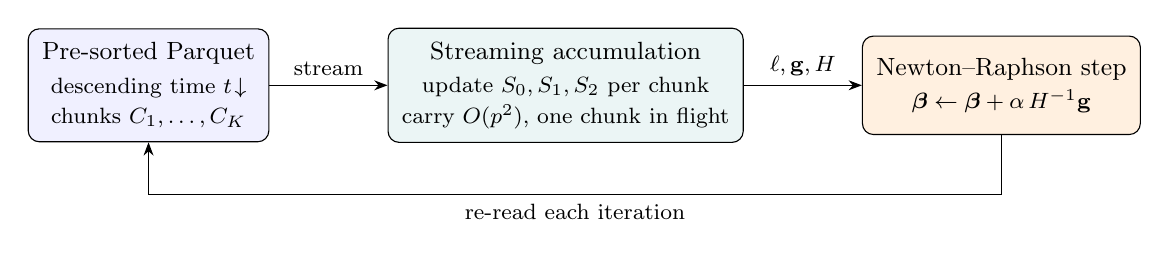
\begin{tikzpicture}[
  font=\small,
  >=Stealth,
  box/.style={draw, rounded corners, align=center, inner sep=5pt,
              minimum height=1.25cm},
]
  \node[box, fill=blue!6, minimum width=2.6cm] (data)
    {Pre-sorted Parquet\\[1pt]\footnotesize descending time $t\!\downarrow$%
     \\\footnotesize chunks $C_1,\dots,C_K$};
  \node[box, fill=teal!8, right=1.5cm of data, minimum width=3.6cm] (acc)
    {Streaming accumulation\\[1pt]\footnotesize update $S_0,S_1,S_2$ per chunk%
     \\\footnotesize carry $O(p^2)$, one chunk in flight};
  \node[box, fill=orange!12, right=1.5cm of acc, minimum width=2.7cm] (nr)
    {Newton--Raphson step\\[1pt]\footnotesize
     $\boldsymbol\beta \leftarrow \boldsymbol\beta + \alpha\,H^{-1}\mathbf{g}$};
  \draw[->] (data) -- node[above]{\footnotesize stream} (acc);
  \draw[->] (acc) -- node[above]{\footnotesize $\ell,\mathbf{g},H$} (nr);
  \draw[->] (nr.south) -- ++(0,-0.75)
            -| node[pos=0.25, below]{\footnotesize re-read each iteration}
            (data.south);
\end{tikzpicture}
\caption{One \coxstream\ Newton--Raphson iteration. A single descending-time
pass streams the pre-sorted Parquet chunk by chunk, updating the risk-set power
sums $S_0,S_1,S_2$; the carry state is $O(p^2)$ and only one chunk is ever
resident, so peak memory is independent of the cohort size $n$. The pass yields
the log-likelihood, score and observed information at the current
$\boldsymbol\beta$; the pass at an accepted trial point also serves the next
iteration, so the data are re-read once per iteration.}
\label{fig:schematic}
\end{figure}

\begin{algorithm}[t]
\caption{One streamed pass at $\boldsymbol\beta$, and the Newton--Raphson step}
\label{alg:coxstream}
\begin{algorithmic}[1]
\Require Parquet chunks in descending time order; current $\boldsymbol\beta$
\Ensure $\ell$, $\mathbf{g}$, $H$ at $\boldsymbol\beta$; the next $\boldsymbol\beta$
\State $S_0, S_1, S_2 \gets 0$; \quad $\ell, \mathbf{g}, H \gets 0$; \quad open tie group $\gets$ empty
\For{each chunk in descending time order}
    \For{each row, in order}
        \If{its time is below the open group's}
            \State close the group: add its $d$ Efron terms to $\ell,\mathbf{g},H$
        \EndIf
        \State add $e^{\mathbf{x}^\top\boldsymbol\beta}(1,\mathbf{x},\mathbf{x}\mathbf{x}^\top)$ to $S_0,S_1,S_2$; if an event, to the group
    \EndFor
\EndFor
\State close the last group
\State $\Delta \gets H^{-1}\mathbf{g}$ \Comment{direct $p\times p$ solve}
\State $\boldsymbol\beta \gets \boldsymbol\beta + \alpha\Delta$, halving $\alpha$ while $\ell$ falls
       \Comment{one pass per trial}
\Statex Start from $\boldsymbol\beta = \mathbf{0}$; the accepted trial's pass
        serves the next iteration, until $\lVert\alpha\Delta\rVert < \CoxStreamTol$.
\end{algorithmic}
\end{algorithm}

\paragraph{Tie correction.} When $d>1$ events share a time $t$, the exact
(permutation) partial likelihood, which averages over every ordering of the
tied events, is expensive for large tie groups, and the Efron approximation
\citep{efron1977efficiency} is the standard. It subtracts a fractional share of
the tied events' contribution from the denominator of each of the $d$ ordered
terms (Appendix~\ref{app:derivation}); \coxstream\ carries the open tie group
across chunk boundaries and finalises it when the group closes, so a streamed
pass computes the same sums as an in-memory Efron pass, up to the rounding of
floating-point addition, even when ties straddle chunks. The open group's moments are $O(p^2)$ whatever its size,
so a large tie group costs no extra memory. Efron is the only tie correction
the packages implement. The cheaper Breslow correction
\citep{breslow1974covariance} reuses the full risk set for all $d$ terms and
can attenuate estimates towards the null when the tied events are a large
share of the risk set.

% ============================================================
\section{Experimental setup}
\label{sec:setup}

\paragraph{Data.} We use synthetic proportional-hazards cohorts with known
coefficients and mutually independent covariates. Event times follow a Weibull
proportional-hazards model with shape \DGPShape; censoring times are
exponential with rate \DGPCensRate\ per year, capped at an administrative
follow-up of \DGPFollowUp\ years, and each subject's time is the earlier of the
two. The ten covariates mimic a clinical cohort (age, sex, treatment, smoking
pack-years, a comorbidity index and five clinical measurements),
with true coefficients between \DGPCoefMin\ and \DGPCoefMax\ in absolute value.
We use a grid of cohort sizes $n$ at fixed $p=\CoxPHNSweepP$ and, from a
separate cohort that adds standard-normal covariates with true coefficient
\DGPExtraCoef, a grid of model widths $p$ at fixed $n = \CoxPHPSweepN$. The
cohorts are stored as Parquet files (a compressed, column-wise on-disk table
format) that hold the response $(t_i, \delta_i)$ and the assembled design
matrix $\mathbf{X}$ (one numeric column per covariate). The benchmark thus
measures the \emph{fitting} cost on a
ready design matrix, the step whose memory grows with $n$ for iterative
in-memory solvers; assembling $\mathbf{X}$ is a separate, streamable step we
discuss in Section~\ref{sec:discussion}. To exercise the Efron tie correction we
use a second cohort of $n = \TiesN$ rows from the same generator, with every
time, event or censoring, rounded up to a whole month, which gives
\TiesNTieGroups\ tied event times with up to \TiesMaxGroupEvents\ events each,
and, as a coarser case, to a whole year. It is written in descending time
order with the rows of each tied time in random order, so that a tied time's
events fall in several chunks. This experiment measures accuracy only, and it
ran on a laptop, not on the instance described below; the archive records its
software versions. In the
timed sweep no two events share a time; the administrative censoring creates
one large group of rows censored at the same time, which contributes no Efron
term.

\paragraph{Baselines and measurement.} We compare against \texttt{lifelines}
(in-memory exact, Python), R \texttt{survival::coxph},
and \texttt{Cyclops} \citep{mittal2014highdim} (in-memory cyclic coordinate
descent, C++ with an R interface; the established large-$n$ Cox tool). All
baselines ran with their default settings and convergence criteria, which
differ from \coxstream's, so their final precision differs slightly; no thread
limits were set. Each method
runs in a fresh subprocess started after the operating system's page cache
(its in-RAM copy of recently read files) has been dropped, so each run reads
its input from disk; the cache is not dropped between the passes of one fit,
so \coxstream's later passes over a file smaller than RAM can be served from
the page cache. Wall time is elapsed time from process start to exit, so it
includes starting the interpreter or R, loading libraries, reading the input
and fitting; we report the median of \CoxStreamReps\ runs for \coxstream\ and
the mean of \BaselineReps\ runs for each baseline. Repeats agreed closely:
within any cell the slowest run took at most \WallSpreadPct\% longer than the
fastest, and the largest RAM added exceeded the smallest by at most
\RAMSpreadPct\%. Memory is measured from
outside the process: a monitor samples its resident set size every \RSSPollMs\,ms, and
we report the \emph{RAM added}, the maximum minus the size at process start,
in binary units (1\,GB is $2^{30}$ bytes).
Measuring from outside counts memory the process's own accounting does not
see, including memory held by the memory allocator and by compiled extensions. It
also counts the language runtime and imported libraries (for the Python
methods, including the benchmark harness's own imports), so comparisons
between Python and R methods include their different fixed memory floors. All
methods read the same copy of the cohort, sorted once by descending time with
\texttt{DuckDB} and written as Parquet in row groups of \CoxStreamChunkRows\
rows. \coxstream\ streams it one row group at a time; the in-memory solvers
load it whole, through the transient copies needed to build each solver's
input structure, and order it as they need inside their timed run. The sort is
done once beforehand and is outside every measurement.

\paragraph{Environment.} Speed and memory were measured on a single Google Cloud
\texttt{\EnvMachine} instance (\EnvVCPUs\ virtual CPUs on \EnvCores\ cores, \EnvCPU,
\EnvRAMGB\,GB RAM, a \EnvDiskGB\,GB persistent disk, Ubuntu \EnvUbuntu) under
Python \EnvPython\ (\texttt{numpy} \EnvNumPy, \texttt{scipy} \EnvSciPy, \texttt{pyarrow}
\EnvPyarrow, \texttt{lifelines} \EnvLifelines, with OpenBLAS) and R \EnvR\
(\texttt{survival} \EnvSurvival, \texttt{Cyclops} \EnvCyclops, with
\EnvRBLAS). We measure resident
memory on Linux rather than macOS deliberately: macOS memory compression
under-reports the resident set and can mask allocation growth, so a Linux host
is needed to gauge the streaming footprint faithfully.

% ============================================================
\section{Results}
\label{sec:results}

\subsection{Exactness}
\coxstream\ reproduces the in-memory estimate: at the comparison cell
($n = \CompetingCoxPHN$, $p=\CoxPHNSweepP$; the one cell at which we quote
head-to-head numbers) its coefficients agree with \texttt{lifelines}
to a maximum gap of $\CoxStreamVsLifelinesCoef$, i.e.\ near machine precision, and the
same MLE is returned by R \texttt{survival::coxph}.
Against the synthetic ground truth the \emph{recovery error}, the largest
absolute difference between a fitted coefficient and the true coefficient that
generated the data, is $\CoxStreamMaxErr$, and every coefficient lies within
\CoxStreamMaxErrSE\ model-based standard errors of its true value: sampling
error, shared by every exact solver. In the Python package inference comes
from the same pass: the observed information $H$ at the estimate is
accumulated in the final streamed pass, so the model-based
standard errors $\sqrt{\mathrm{diag}(H^{-1})}$ (the inverse observed partial
information, as \texttt{coxph} and \texttt{lifelines} report without a robust
option) cost no extra pass over the data. At the comparison cell they agree
with those of \texttt{lifelines} to a maximum relative difference of
$\CoxStreamVsLifelinesSERel$, and the Python test suite checks them against an
independent in-memory Efron information matrix. Robust (sandwich) variances
are not provided.

The Efron correction is reproduced across chunk boundaries as well. On the
tied cohort with chunks of \TiesRowGroupMin\ rows, every one of the
\TiesNTieGroups\ tied event times has its events split across chunks. We
fitted the monthly grid at chunk sizes from \TiesRowGroupMin\ rows to the
whole file in one chunk, the yearly grid at chunk sizes in between, and a
subsample of \TiesSubN\ rows down to single-row chunks. In every one of these
fits the streamed coefficients agree with an in-memory Efron fit by R
\texttt{survival::coxph} to within $\TiesStreamVsEfronCoef$, and the standard
errors to a relative $\TiesStreamVsEfronSERel$. Most of that residual lies with
the R reference, not with the streaming: the Efron fit of \texttt{lifelines}
differs from that of R by $\TiesRVsLifelinesCoef$, whereas the stream agrees
with \texttt{lifelines} to $\TiesStreamVsLifelinesCoef$, and on the subsample a
direct implementation of the textbook formulas matches the stream to
$\TiesStreamVsNumpyCoef$. A Breslow fit of the same data differs from the Efron
fit by $\TiesBresVsEfronMonthly$ on the monthly grid and
$\TiesBresVsEfronYearly$ on the yearly one, orders of magnitude more, so the
experiment does tell the two corrections apart.

\paragraph{Model width.} At fixed $n = \CoxPHPSweepN$ we also fitted models of
$p = \CoxPHPLo$ to $\CoxPHPHi$ covariates, from a cohort in which all
$\CoxPHPHi$ have real effects. \texttt{lifelines} and R
\texttt{survival::coxph}, fitted at every width, return the same recovery
error as \coxstream\ at each. That error falls from $\CoxStreamErrLoP$ at
$p=\CoxPHPLo$ to $\CoxStreamErrHiP$ at $p=\CoxPHPHi$ because a model that
omits covariates with real effects attenuates the coefficients it keeps, the
non-collapsibility of the Cox model
\citep{gail1984biased,struthers1986omitted}, not because of any
implementation. The two in-memory references of this sweep were fitted on a
laptop, not on the measurement instance, so only their coefficients are used
and wall time as a function of $p$ is not compared between methods.

\subsection{Scaling: memory and speed}
Memory is the main result. \coxstream's RAM added is essentially flat in $n$:
across a $\CoxStreamRAMNFactor\times$ increase in cohort size (from $n =
\CoxStreamRAMLoN$ to $n = \CoxStreamRAMHiN$) it stays between
\CoxStreamRAMMinGB\ and \CoxStreamRAMMaxGB\,GB, because the carry state is
$O(p^2)$ and only one chunk is resident at a time. \texttt{lifelines} holds the
full design matrix, so its memory grows with $n$: at $n = \CoxPHRAMRatioN$ it
adds \LifelinesRAMGB\,GB, more than ten times the RAM of \coxstream\
(Figure~\ref{fig:ram}). The in-memory baselines were run up to $n =
\CoxPHRAMRatioN$ by design, not because they failed, and their footprint grows
linearly with $n$ above a fixed floor. Continued along its measured straight
line to the $\ExtrapN$ rows of the largest registries, \texttt{lifelines}
would need about \LifelinesRAMExtrapGB\,GB, whereas \coxstream's footprint is
set by the chunk size and $p$.

\begin{figure}[t]
\centering
\includegraphics[width=0.7\textwidth]{figures/coxph_ram_scaling}
\caption{RAM added (peak resident set size minus the size at process start)
versus $n$ ($p=\CoxPHNSweepP$; median of \CoxStreamReps\ runs for \coxstream,
mean of \BaselineReps\ for each baseline; linear axes). \coxstream\ is flat in
$n$; the in-memory solvers (\texttt{lifelines}, R \texttt{survival::coxph},
\texttt{Cyclops}) grow linearly with the cohort. The baselines were run up to
$n = \CoxPHRAMRatioN$ and \coxstream\ further; lines are not clipped to a common
range.}
\label{fig:ram}
\end{figure}

\paragraph{Speed.} In our benchmark at $p = \CoxPHNSweepP$, holding memory flat
does not cost wall time (the one-off sort excluded), and \coxstream\ remains
faster than a strong baseline. \texttt{lifelines} is slow; \texttt{Cyclops}
\citep{mittal2014highdim}, purpose-built for large-$n$ Cox, fits the same MLE
\CyclopsVsLifelinesSpeedup\ times faster than \texttt{lifelines} at the
comparison cell. Against \emph{that} baseline
\coxstream\ is still \CoxStreamVsCyclopsSpeedup\ times faster there
(\LifelinesVsCoxStreamSpeedup\ times faster than \texttt{lifelines};
Figure~\ref{fig:time}). Each streamed pass is a single $O(n)$ sequential scan
with $O(p^2)$ work per row in compiled code; we did not profile the baselines,
so we do not attribute the gaps to particular causes. Every
timed \coxstream\ fit at $p = \CoxPHNSweepP$, from the smallest $n$ to the
largest, converged in \CoxStreamIters\ iterations and \CoxStreamPasses\ passes
over the data, and no fit in either sweep needed step-halving. The timed code
therefore behaves as the released package does: the two differ only in the
convergence flag after an exhausted step-halving, a branch no timed fit reached.
\texttt{Cyclops} is exact too: it recovers the same true coefficients (error
$\CyclopsMaxErr$, matching every exact solver) and agrees with
\texttt{lifelines} to $\CyclopsVsLifelinesCoef$, within its default
convergence criterion. However, holding the cohort in memory, it uses
$\CyclopsRAMRatio$ times the RAM of \coxstream, and its footprint grows with
$n$ (Figure~\ref{fig:ram}). R \texttt{survival::coxph}, the reference
implementation most readers reach for, uses $\RSurvivalRAMRatio$ times the RAM
of \coxstream\ at the same comparison cell (Figures~\ref{fig:ram}
and~\ref{fig:time}). Figure~\ref{fig:scatter} shows memory and time together.

\begin{figure}[t]
\centering
\includegraphics[width=0.7\textwidth]{figures/coxph_time_scaling}
\caption{Wall time, from process start to exit, versus $n$
($p=\CoxPHNSweepP$; median of \CoxStreamReps\ runs for \coxstream, mean of
\BaselineReps\ for each baseline; log $y$-axis, linear $n$-axis). The baselines
were run up to $n = \CoxPHRAMRatioN$ and \coxstream\ further. \coxstream\ is
fastest at every $n$; \texttt{Cyclops}, though faster than \texttt{lifelines}
and R \texttt{survival::coxph}, stays above \coxstream\ throughout.}
\label{fig:time}
\end{figure}

\begin{figure}[t]
\centering
\includegraphics[width=0.7\textwidth]{figures/coxph_efficiency_scatter}
\caption{RAM added (peak resident set size minus the size at process start)
versus wall time at $p=\CoxPHNSweepP$, one point per method and $n$ (labels
give $n$ in millions; both axes logarithmic; median of \CoxStreamReps\ runs for
\coxstream, mean of \BaselineReps\ for each baseline). The baselines were run
up to $n = \CoxPHRAMRatioN$ and \coxstream\ further. \coxstream\ occupies the
low-memory, low-time corner at every $n$.}
\label{fig:scatter}
\end{figure}

% ============================================================
\section{Discussion and limitations}
\label{sec:discussion}

\coxstream\ makes the working memory of exact Cox regression a function of $p$
and the chunk size, not of $n$: a cohort for which an in-memory solver would
need RAM that grows with its size fits in a fixed footprint, while the wall
time still grows linearly with $n$.

\paragraph{Assembling the design matrix.} \coxstream\ fits from a stored design
matrix; it does not build one, and the benchmarks measure the fit alone. This
separation is deliberate. Constructing $\mathbf{X}$ from raw records, which means
encoding categorical variables, forming interactions and standardising columns, is a
row-wise transform: each row's features depend only on that row, so $\mathbf{X}$
can be written to disk one chunk at a time. The global reductions it needs
(column means and standard deviations for standardisation, and the levels of
each categorical variable) take one streaming pass, with memory proportional
to $p$ and the number of levels, not to $n$. Assembly therefore
need not hold the cohort in
memory either, and it is paid once. The fit is where an in-memory solver's
footprint grows with $n$, because it holds the full design matrix resident in RAM
across every iteration; \coxstream's per-iteration re-read comes from disk
instead, removing that resident cost.

\paragraph{Repeated fits.} The saving would compound when one design matrix
is fitted many times, as in bootstrap resampling or cross-validation: the
streaming pass extends naturally to nonnegative case weights (a bootstrap
multiplicity, a fold mask) applied on the fly, keeping working memory $O(p^2)$
across refits. Case weights are not implemented in the current packages, and
with tied times a weighted Efron fit is not the same as a fit to replicated
rows; a systematic study is left to future work.

\paragraph{Assumptions and limitations.} The estimator needs a complete-case,
numeric design matrix: missing values must be resolved during assembly, and
the Python package rejects missing or infinite durations and covariates (the
event column is not checked, and must hold only 0 and 1). Collinear covariates
make $H$ singular and the Newton solve fail, as for any exact Cox fitter
without aliasing detection, and separated data have no finite maximiser. The
packages return the coefficients, their model-based covariance and convergence
information; they compute no baseline hazard, predicted survival, residuals or
concordance, so proportional-hazards diagnostics need other tools. The current
scope is the right-censored Cox model with fixed covariates and time since
origin as the time scale. Not supported: strata, case weights and offsets, left
truncation (delayed entry), time-varying covariates and counting-process
$(\mathrm{start}, \mathrm{stop}]$ data, robust or clustered variances, and
competing risks; the \texttt{start} and \texttt{stop} arguments of the Python
\texttt{fit} only form the duration $\mathrm{stop} - \mathrm{start}$. Left
truncation does not fit the same accumulation unchanged: in a descending pass a
subject must leave the risk set once the time falls below its entry time, so
the sums no longer only grow. \texttt{Cyclops}'s GPU implementation, by
contrast, fits stratified and time-varying Cox models \citep{yang2023gpu}.
Only the Parquet entry points
(\texttt{fit\_parquet} in Python, \texttt{coxstream\_arrow} in R) are out of
core; the in-memory \texttt{fit} and the R formula interface hold the design
matrix. The input must be sorted by descending time beforehand, a one-off
external sort whose cost our benchmarks do not include. Every cohort file in
our benchmark was also smaller than the machine's RAM, so the passes after the
first could be served from the page cache; we have not timed a file that must
be re-read from disk on every pass, where the wall time, though not the
memory, will depend on the disk. Two further limits bound the method. It
re-reads the data on every iteration, so a stream that cannot be re-read needs
an approximate single-pass method instead. And the carry state is $O(p^2)$, so
wide models ($p$ in the hundreds) are expected to make the $p \times p$
observed information, not the data, the bottleneck; we have not compared wall
time in $p$ between methods. When the cohort fits in memory, or the analysis
needs strata, delayed entry or time-varying covariates, an in-memory solver
such as \texttt{survival::coxph} remains the right tool.

% ============================================================
\section{Conclusion}
\label{sec:conclusion}

\coxstream\ computes the Efron partial-likelihood estimate of the Cox model
out of core, in working memory independent of the cohort size, matching
in-memory solvers to near machine precision and carrying the Efron tie
correction exactly across chunk boundaries. In our benchmark ($p =
\CoxPHNSweepP$, sort excluded) it was faster than the in-memory baselines, and
its memory stayed flat in $n$, where theirs grew with the cohort. Its input
must first be sorted by descending time, and strata, left truncation,
time-varying covariates and case weights are not yet supported.

% ============================================================
\section*{Code and data availability}

\coxstream\ is open source under the MIT licence (the R package also vendors
the Apache-2.0 Arrow C Data and Stream interface header) and packaged for both
ecosystems: a Python package on PyPI (\texttt{pip install "coxstream[parquet]"},
which adds the \texttt{pyarrow} reader the out-of-core fit needs;
\url{https://github.com/tommycarstensen/coxstream}) and an R package on CRAN
(\texttt{install.packages(c("coxstream", "arrow"))}, \texttt{arrow} being needed
for the out-of-core fit; \url{https://github.com/tommycarstensen/coxstream-r}),
with releases archived on Zenodo \citep{coxstream2026,coxstreamr2026}. Both
implement the same streaming accumulation with the Efron tie correction;
step-halving, centring, the check for missing values, the non-convergence
warning, the covariance at the final estimate and the sort check are in the
Python package (Section~\ref{sec:method}). The Python test suite
checks coefficients, standard errors and tie groups split across chunks against
an independent in-memory Efron implementation; the R test suite checks
coefficients against \texttt{survival::coxph}, including on tied data.

What is needed to reproduce the results is in a separate archive
\citep{coxstreampaper2026}: the benchmark harness, the seeded data generator,
the result files from which every number and figure in this paper is
generated, the record of the measurement machine and its package versions, and
both packages as they were measured. All data in this paper are synthetic
Weibull proportional-hazards cohorts, so the cohorts themselves are not
deposited: the generator recreates them from the seed. Rebuilding the paper
from the result files takes minutes on any machine and rerunning the tie
experiment takes minutes on a laptop; rerunning the speed and memory benchmark
takes hours on a Linux machine, and its timings depend on the hardware.

% ============================================================
\appendix
\section{Score and observed information}
\label{app:derivation}

Write $\eta_i = \mathbf{x}_i^\top\boldsymbol\beta$ and $w_i = e^{\eta_i}$, and let
$S_0(t), S_1(t), S_2(t)$ be the risk-set power sums of
Eq.~\eqref{eq:powersums}. For distinct event times, the partial log-likelihood,
score, and observed information are
\begin{align}
  \ell(\boldsymbol\beta) &= \sum_{i:\,\delta_i=1}
      \bigl[\eta_i - \log S_0(t_i)\bigr], \\
  \mathbf{g}(\boldsymbol\beta)
      = \frac{\partial\ell}{\partial\boldsymbol\beta}
      &= \sum_{i:\,\delta_i=1}
         \Bigl[\mathbf{x}_i - \tfrac{S_1(t_i)}{S_0(t_i)}\Bigr], \\
  H(\boldsymbol\beta)
      = -\frac{\partial^2\ell}
              {\partial\boldsymbol\beta\,\partial\boldsymbol\beta^\top}
      &= \sum_{i:\,\delta_i=1}
         \Bigl[\tfrac{S_2(t_i)}{S_0(t_i)}
               - \tfrac{S_1(t_i)}{S_0(t_i)}\tfrac{S_1(t_i)^\top}{S_0(t_i)}
         \Bigr].
\end{align}
Under the risk-set distribution that weights subject $j$ by $w_j / S_0(t_i)$,
the score summand is $\mathbf{x}_i$ minus the mean of the covariates and the
information summand is their covariance. $H$ is therefore a sum of covariance
matrices, hence positive semidefinite, and positive definite when the
covariates are not collinear over the risk sets of the observed events.

\paragraph{Efron tie correction.} When $d > 1$ events share a time $t$, let $D$
index the tied events and $s_0 = \sum_{j \in D} w_j$,
$s_1 = \sum_{j \in D} w_j\mathbf{x}_j$,
$s_2 = \sum_{j \in D} w_j\mathbf{x}_j\mathbf{x}_j^\top$ denote their own
moments, with $S_r = S_r(t)$ the risk-set sums over every row with time at
least $t$, censored rows at $t$ included. The Efron approximation
\citep{efron1977efficiency} replaces the single risk-set denominator by the $d$
terms $S_r - \tfrac{k}{d}\,s_r$ for $k = 0,\dots,d-1$ ($r \in \{0,1,2\}$),
averaging over the unknown order of the tied events. Writing
$\mathbf{m}_k = (S_1 - \tfrac{k}{d}s_1)/(S_0 - \tfrac{k}{d}s_0)$, the group
contributes
\begin{align}
  \ell_D &= \sum_{i \in D} \eta_i
            - \sum_{k=0}^{d-1} \log\bigl(S_0 - \tfrac{k}{d}s_0\bigr), \\
  \mathbf{g}_D &= \sum_{i \in D} \mathbf{x}_i - \sum_{k=0}^{d-1} \mathbf{m}_k, \\
  H_D &= \sum_{k=0}^{d-1}
         \Bigl[\frac{S_2 - \tfrac{k}{d}s_2}{S_0 - \tfrac{k}{d}s_0}
               - \mathbf{m}_k\mathbf{m}_k^\top\Bigr].
\end{align}
Each summand of $H_D$ is again a covariance matrix, under weights $w_j$ outside
$D$ and $(1 - \tfrac{k}{d})\,w_j$ inside it, so $H$ stays positive
semidefinite with ties. \coxstream\ accumulates $S_0, S_1, S_2$ up to and
including the group and the tied moments $s_0, s_1, s_2$ within it, and closes
the group only when a strictly earlier time arrives or the data end, so the
correction is carried exactly even when a tie group spans a chunk boundary.
For distinct times ($d = 1$) it reduces to the expressions above.

\bibliographystyle{plainnat}
\bibliography{paper}

\end{document}
